% Motivation
%

\chapter{Einleitung}

\begin{figure}[!htb]
	\centering
	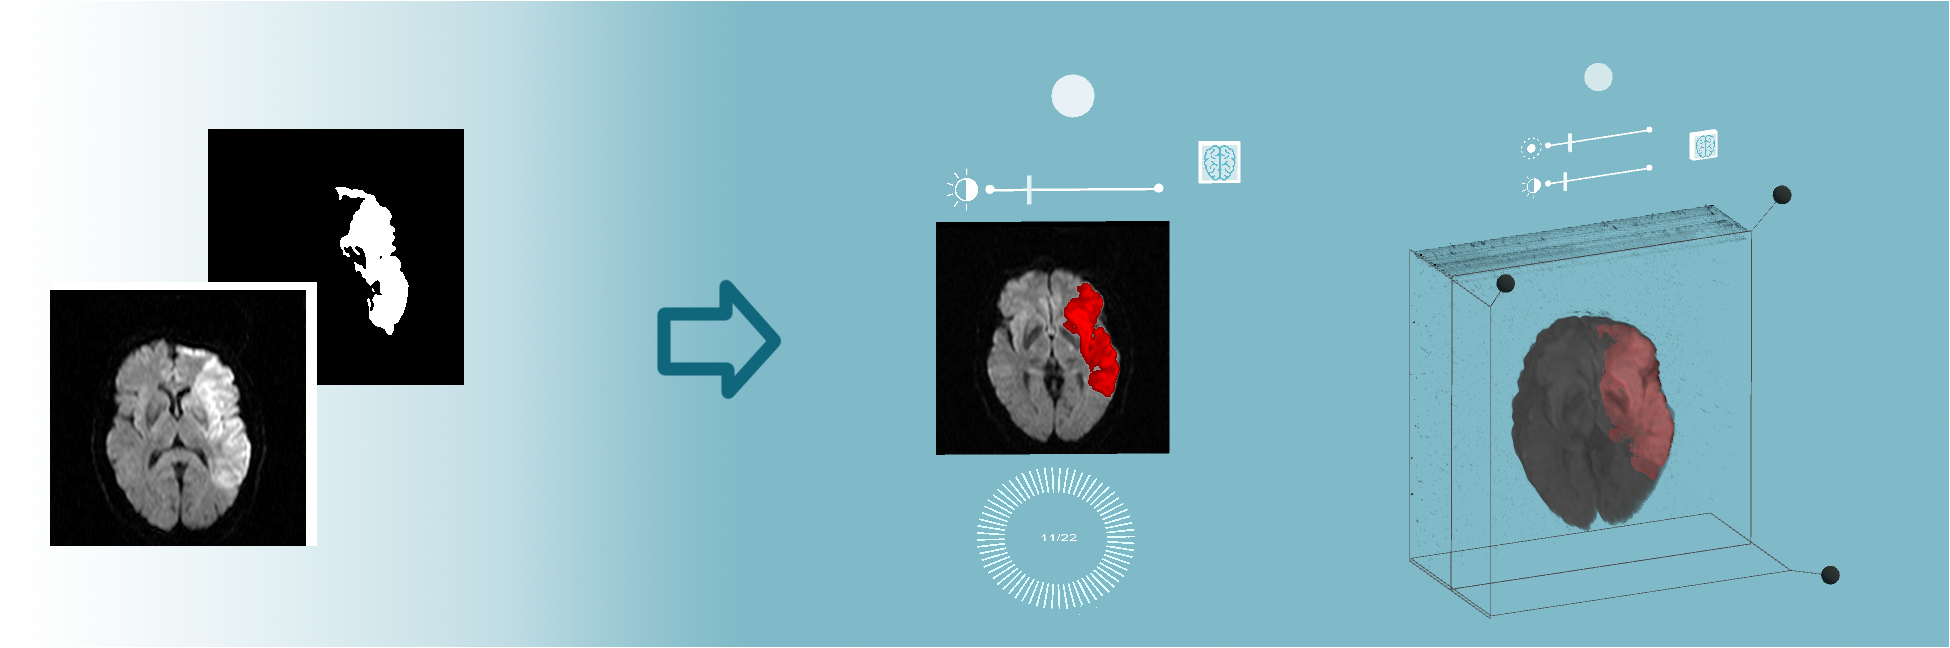
\includegraphics[width=1\linewidth]{images/teaser.png}
	\caption{}
	\label{img:teaser}
\end{figure}


Der Einsatz von MRTs\footnote{ Magnetresonanztomographie, Erläuterung in Abschnitt \ref{mrt}} ermöglicht es Ärzten einen Einblick in das innere des menschlichen Körpers zu erlangen, ohne diesen dabei zu verletzten. Sie erhalten Bilder innerer Organe, anhand derer sich dessen Aufbau und Funktionalität beobachten lassen. Aber auch mögliche Fehlfunktionen oder Anomalien können so erfasst werden. So können auf MRT-Scans gebrochene Knochen, innere Verletzungen oder Schlaganfälle erkannt und beurteilt werden. Im Fall von Schlaganfällen kann ein MRT aufzeigen welcher Bereich des Gehirns von diesem betroffen ist, und welchen Umfang der Schaden hat.
% Wie genau?
Um den Fall eines Patienten richtig beurteilen zu können ist es unabdingbar, dass der Arzt eine möglichst umfassende Vorstellung von der Struktur des Gehirns des Patienten und vor allem von den vom Schlaganfall betroffenen Bereichen hat. Nur wenn dies der Fall ist, kann eine sinnvolle Diagnose und Behandlung angewandt werden.
In diesem sowie vielen anderen Anwendungsfällen kann die Visualisierung der MRT-Bilder in einer AR-Anwendung zu einem besseren Verständnis der Lage führen. Die intuitive Interaktion mit diesen würde dies zusätzlich unterstützen. 
Diese Arbeit untersucht, inwiefern eine dreidimensionale Darstellung der Daten in einer interaktiven AR-Anwendung die Einschätzung von und den Umgang mit den MRT-Daten verbessert. Der Fokus liegt dabei auf dem Einsatz in der Schlaganfalldiagnose und -behandlung.  
%Diese Arbeit stellt die Möglichkeit vor den Umgang mit MRT-Daten anschaulicher und intuitiver zu gestalten, um somit die Arbeit von Radiologen im Bereich der Schlaganfallbehandlung zu erleichtern und die Gesundheit ihrer Patienten zu verbessern.



\section{Motivation}
\label{motivation}

Um MRT-Scans zu studieren benutzen Ärzte in der Regel speziell dafür entwickelte Software. Diese stellt meist Querschnitte des Gehirns aus drei verschiedenen Blickwinkeln dar, sodass es von allen Seiten zusehen ist. Entlang dieser Sichtachsen kann der Nutzer die Ansicht durch die Schichten des Scans bewegen. Die aktuelle Position der gerade angezeigten Schicht kann in den anderen Achsenansichten farbig eingezeichnet werden, um dem Nutzer ein möglichst umfassendes Bild des gescannten Gehirns zu vermitteln. 
Beispiele für solche Software werden im Abschnitt \ref{radiologieSoftware} näher erläutert.

Die zweidimensionale Ansicht, in der die Bilder vorliegen, können allerdings eine falsche Vorstellung von der vorliegenden Situation schaffen. 
Durch die Reduzierung um eine Dimension entsteht ein verzerrtes Bild des Gehirns. Die Darstellung der verschiedenen Achsen auf den Scans soll den Arzt bei der Orientierung unterstützen. Da das Gehirn allerdings durch mehrere Bilder dargestellt wird, ist es diesem nicht möglich den Zustand auf einen Blick zu erfassen. Stattdessen müssen die Informationen aus zwei oder mehr Bildern im Kopf zusammengesetzt werden, was ein gewisses räumliches Vorstellungsvermögen voraussetzt. Dies ist ein kognitiver Aufwand, der Ärzte zusätzlich belastet während sie sich darauf konzentrieren Anomalien in den Scans eines Patienten zu erkennen und einzuschätzen. Um aus den Bildern ein zutreffendes Verständnis der Lage ableiten zu können bedarf es zudem Übung im Umgang mit MRT-Daten, welche nicht bei jedem Arzt in gleichem Maße vorausgesetzt werden kann.

Wird auf einem Scan ein Schlaganfall entdeckt, ist es durch die Abstraktion des Organs schwierig eine korrekte Vorstellung von der Größe und Lage des betroffenen Bereichs zu bekommen, da jeweils nur eine Schicht des Gehirns sichtbar ist. 
Eine dreidimensionale Ansicht des gescannten Gehirns würde einen sehr viel deutlicheren Einblick in den Zustand des Patienten liefern. Vor allem der vom Schlaganfall betroffene Bereich, den der Arzt kennzeichnet, wäre in 3D um einiges anschaulicher. Durch die bessere Einschätzung von Lage und Größe des betroffenen Bereichs fällt es leichter nachzuvollziehen, welche Bereiche des Gehirns betroffen sind und welche Auswirkungen der Schlaganfall auf den Patienten hat. Dies ist nicht nur für den behandelnden Arzt hilfreich. Durch die klare und eindeutige Darstellung kann die Situation auch leichter anderen Personen erläutert werden. Dies trifft auf Patienten oder andere Ärzte zu, die der behandelnde Arzt eventuell in den Fall mit einbeziehen möchte.
Schließlich würde eine 3D-Darstellung auch das Verständnis in Lernzwecken begünstigen. 
Da der betroffene Bereich in einer 3D-Darstellung auf einen Blick erfasst werden kann, eignet sie sich außerdem, um den direkten Vergleich zwischen zwei Zuständen zu ziehen. So fiele es leichter beispielsweise die Größe des Bereichs vor und nach einer Therapie gegenüberzustellen, um deren Erfolgt zu demonstrieren oder zu beurteilen.
Auch Voraussagen von Therapieerfolgen könnten anschaulich demonstriert werden.

% UX  
% Software zum Vergleichen finden
Um die Anschaulichkeit und Plastizität der 3D-Darstellung voll zur Geltung zu bringen muss sie auch im dreidimensionalen Raum platziert werden. Eine volumetrische Darstellung der Daten in einer Bildschirmanwendung ist nur eine Projektion auf eine zweidimensionale Fläche. Die Darstellung wird dabei abstrahiert und der Nutzer kann nicht direkt mit dem Objekt interagieren.
Die Platzierung der dreidimensionalen MRT-Darstellung in der dreidimensionalen Welt des Nutzers löst diese Barrieren auf. AR- und VR-Technologien\footnote{Augemented und Virtual Reality, Erläuterung in Abschnitt \ref{arVr}} ermöglichen sowohl die Visualisierung von dreidimensionalen virtuellen Objekten in der Umgebung des Nutzers, als auch die direkte Interaktion mit diesen. Diese gestaltet sich dabei auch deutlich intuitiver als die Bedienung eines Programms mit konventionellen Eingabemodulen, wie z.B. einer Maus. Das trifft vor allem auf tragbare AR-Brillen zu, deren Steuerung in der Regel ohne externe Steuerungsgeräte, wie Controller erfolgt. Dies ermöglicht eine verständliche und schnelle Bedienung, was ungeübten Nutzern, wie z.B. einem Patienten oder Studenten zu Gute kommt. Die Nutzung der Anwendung wird dadurch zudem interessanter und unterhaltsamer.

Die Steuerung durch die Hände des Nutzers ist im medizinischen Bereich außerdem von besonderem Wert. So kann die Anwendung auch in sterilen Räumen oder sogar während einer Operation eingesetzt werden. In diesem Szenario kommt ein weiterer Vorteil eines tragbaren AR-Headsets zur Geltung: Durch das transparente Display ist es dem Nutzer möglich während der Nutzung der Anwendung seine Umgebung im Auge zu behalten. 
Eine AR-Anwendung ermöglicht es also einem Arzt während einer Operation oder einem neuroradiologischen Eingriff relevante Daten abzurufen.
Auch für Einsatz zu Lernzwecken ist eine AR-Anwendung besser geeignet, da sie die Kommunikation zwischen Lernenden und Lehrenden erlaubt.
Durch die kabellosen, tragbaren AR-Headsets ist gleichzeitig eine höhere Mobilität gegeben, als durch einen Desktop-PC. Dadurch kann die Anwendung unabhängig von der Umgebung überall zum Einsatz kommen, wie z.B. in (interdisziplinären) Fallbesprechungen oder während einer Patientenvisite.. 
Die Vorteile einer AR-Anwendung werden im Kapitel \ref{konzept} noch einmal erläutert.

AR-Anwendungen entwickeln sich stetig weiter und werden in der Zukunft einen immer größeren Teil des Alltags einnehmen \cite{forbes}. Diese Entwicklung wird sich voraussichtlich auch auf den medizinischen Bereich auswirken. 
Ärzte sind sich der neuen Möglichkeiten bewusst und sind daran interessiert, 
in welchen Einsatzgebieten man einen Nutzen aus diesen ziehen kann, wie \cite{holomed1} zeigen.

All diese Gründe sprechen dafür, dass eine Darstellung von MRT-Volumen innerhalb einer AR-Anwendung Vorteile mit sich bringt, die die Arbeit mit MRT-Scans in vielen Bereichen verbessern kann. Diese sind im Folgenden zusammengefasst.

\begin{itemize}
\item 3D-Darstellung der MRT-Daten verbessert allgemeines Verständnis 
\item Direkte Interaktion mit Daten ermöglicht intuitive und ansprechende Interaktion
\item Handsteuerung und Portabilität einer AR-Anwendung ermöglichen Gebrauch im OP
\end{itemize}

\section{Zielsetzung}
% hier techniken kokretisieren

Ziel dieser Arbeit ist es zu untersuchen inwiefern die im vorherigen Abschnitt dargelegten Vorteile einer AR-Anwendung zur Visualisierung von MRT-Daten die Arbeit von Ärzten bereichern können.
Hierzu soll eine prototypische Anwendung konzipiert und implementiert werden, die die eben genannten Möglichkeiten demonstriert: mARt. 
Der Fokus liegt dabei auf auf der Darstellung und Untersuchung von Gehirnscans, die in der Schlaganfalldiagnose und -behandlung verwendet werden.
Um eine nützliche Anwendung zu entwickeln, die den Anforderungen eines Einsatzes in diesem Bereich entspricht, werden Interviews mit einem Neurologen geführt werden. Aus diesen wird dann die nötige Funktionalität der Anwendung abgeleitet. 
Schließlich wird die Anwendung evaluiert, um Aufschluss darüber zu geben, ob die Untersuchung von MRT-Scans von ihrem Einsatz profitiert.
Die Anwendung ist dabei nicht als einsetzbares Produkt zu verstehen sondern als Prototyp, der die Nützlichkeit und das Potenzial des Programms beweisen soll.

\section{Struktur dieser Arbeit}

Zuerst werden im  Kapitel \ref{grundlagen} theoretische Grundlagen zu Methoden und Techniken erläutert, die für das Verständnis dieser Arbeit notwendig bzw. hilfreich sind. Weiterhin werden andere Arbeiten vorgestellt,die sich mit einem ähnlichem Thema befassen oder die inhaltlich die Thematik dieser Arbeit berühren.
Um die genaue Funktionalität und den Umfang der zu implementierenden Anwendung festzustellen, werden in Kapitel \ref{anforderung} die bereits erwähnten Interviews mit einem Radiologen ausgewertet und daraus User Stories und schließlich eine Anforderungsliste erstellt.
Anhand dieser Anforderungen wird in Kapitel \ref{konzept} ein theoretischer Entwurf der Anwendung ausgearbeitet, indem Methoden und Techniken, sowie die Benutzung des Programms diskutiert und konzipiert werden.
Die Umsetzung des entwickelten Konzeptes wird schließlich in Kapitel \ref{implementierung} beschrieben. Dabei wird auch auf Hürden eingegangen, die im Rahmen dieser auftraten.
Das Ergebnis der Implementierung wird in Abschnitt \ref{ergebnisse} dargelegt.
Die Anwendung wird anschließend getestet und mit den zuvor gestellten Anforderungen verglichen. Die Resultate dessen werden in Kapitel \ref{evaluation} beschrieben. 
In Kapitel \ref{fazit} werden die Schwerpunkte der Arbeit noch einmal zusammengefasst und mögliche Weiterentwicklungen in der Zukunft werden diskutiert. 
 